\chapter{Theoretical Foundations\label{theoretical_foundations}}
% 中文版：
% \chapter{理论基础\label{theoretical_foundations}}
% 本章将介绍本工程的两个理论基础：
% \begin{itemize}
%     \item rtabmap的工作原理
%     \item ROS2工作框架
% \end{itemize}
% 因篇幅有限，本文仅对俩理论基础中的核心内容进行部分介绍，如需了解更多内容，请参考相关文献\citep{rtabmap,labbe2024memory,ros2humble}。
% English version:
Simultaneous localization and mapping (SLAM) \citep{dissanayake2001solution} is the capability required by robots to build and update a map of its operating environment and to localize itself in it. A key feature in SLAM is to recognize previously visited locations. This process is also known as loop closure detection, referring to the fact that coming back to a previously visited location makes it possible to associate this location with another one recently visited.

This chapter will introduce the theoretical foundations of the engineering project, which mainly includes the following contents:
\begin{itemize}
    \item The working principle of RTAB-Map
    \item The ROS2 working framework
\end{itemize}

\section{RTAB-Map Working Principle\label{sec:rtabmap_working_principle}}

% 中文版：
% \subsection{RTAB-Map工作原理\label{sec:rtabmap_working_principle}}
% 首先介绍本工程的第一个理论基础——RTAB-Map (Real-Time Appearance-Based Mapping)，这是一种基于深度、立体和雷达图的增量外观环路闭合检测器的SLAM方法\citep{rtabmap}。在本工程中，SLAM方法仅基于立体相机图，是一种纯视觉SLAM方法。关于它的原理，这里只重点介绍\citep{labbe2024memory}中介绍的内存管理相关的部分。
% English version:
Firstly, the first theoretical foundation of this engineering project is introduced: RTAB-Map (Real-Time Appearance-Based Mapping), which is a RGB-D, Stereo and Lidar Graph-Based SLAM approach based on an incremental appearance-based loop closure detector \citep{rtabmap}. In this engineering project, the SLAM method is only based on the stereo camera graph, which is a purely visual SLAM approach. Regarding its principles, this section will focus on the memory management aspects introduced in \citep{labbe2024memory}.

For global loop closure detection approaches \citep{newman2006outdoor,cummins2008fabmap,angeli2008incremental,botterill2011bow,konolige2010view}, a general way to detect a loop closure is to compare a new location with the ones associated with previously visited locations. If no match is found, then a new location is added. A problem with this approach is that the amount of time required to process new observations increases with the number of locations in the map. If this becomes larger than the acquisition time, a delay is introduced, leading to an obsolete map. In addition, a robot operating in large areas for a long period of time will ultimately build a very large map, making updating and processing the map difficult to achieve in real-time.

The idea of RTAB-Map resides in only using a certain number of locations for loop closure detection so that real-time constraint can be satisfied, while still having access to the locations of the entire map when necessary. When the number of locations in the map makes processing cycle time for finding matches greater than a real-time threshold, this approach transfers locations less likely to cause loop closure detection from the robot’s \textbf{Working Memory (WM)} to \textbf{Long Term Memory (LTM)}, so that they do not take part in the detection of loop closures. However, if a loop closure is detected, neighbor locations can be retrieved and brought back into \textbf{WM} to be considered in loop closure detections. This mechanism can be seen as a dynamic way to generate and to dynamically maintain a constant number of locations in \textbf{WM}.

In order to keep in \textbf{WM} the locations that are more susceptible to be revisited, RTAB-Map evaluates the number of times a location has been matched or consecutively viewed (referred to as \textbf{Rehearsal}) to set its weight, making it possible to prioritize the locations seen more often than others and that are more likely to cause loop closures. When transfer occurs, the location with the lowest weight is selected. If there are locations with the same weight, then the oldest one is selected to be transferred to \textbf{LTM}.

Similar to \citep{angeli2008incremental}, locations in the \textbf{Short Term Memory (STM)} are not used for loop closure detection, to avoid loop closure detection on locations that have just been visited (the last location always looks similar to the most recent ones). \textbf{STM} size is fixed based on the robot velocity and the rate at which the locations are acquired. When the number of locations reaches \textbf{STM} size limit, the oldest location is moved into \textbf{WM}.

Figure~\ref{fig:rtabmap_memory_management} illustrates the overall loop closure detection process which is explained in details in the following subsections.

\begin{figure}[htbp]
    \centering
    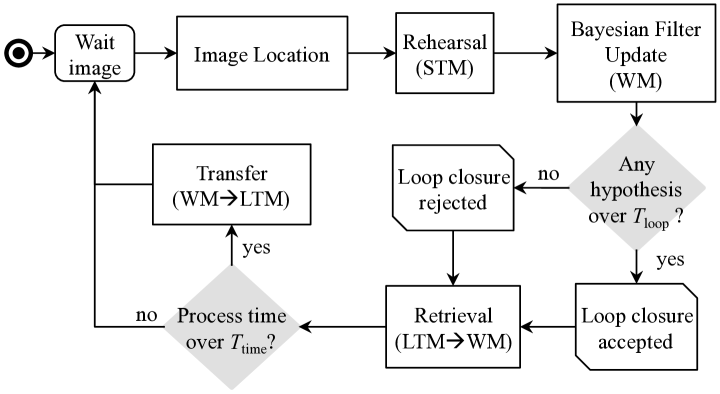
\includegraphics[width=0.9\textwidth]{figs/theory/rtabmap_memory_management.png}
    \caption{Flow chart of RTAB-Map memory management loop closure detection processing cycle.}
    \label{fig:rtabmap_memory_management}
\end{figure}

\subsection{Image Location}
\label{sec:image_location}
The bag-of-words approach \citep{sivic2003videogoogle} is used to create a signature $z_t$ of an image acquired at time $t$. An image signature is represented by a set of visual words contained in a visual dictionary incrementally constructed online using a randomized forest of kd-trees \citep{muja2009flann}. Speeded-Up Robust Features (SURF) \citep{bay2008surf} are extracted from the image as the visual words. A location $L_t$ is then created with signature $z_t$, a weight initialized to 0, and a bidirectional link in the graph with the previous location $L_{t-1}$. The dictionary contains only words of locations in \textbf{WM} and \textbf{STM}.

\subsection{Rehearsal}
\label{sec:rehearsal}
To update the weight of the acquired location, $L_t$ is compared to the ones in \textbf{STM} from the most recent ones to the latest, and similarity $\mathfrak{S}$ is evaluated using equation~(\ref{eq:similarity}):

\begin{equation}
    \label{eq:similarity}
    \mathfrak{S}(z_t, z_c) =
    \begin{cases}
        \dfrac{N_{\text{pair}}}{N_{z_t}}, & \text{if}\,\, N_{z_t} \ge N_{z_c} \\
        \dfrac{N_{\text{pair}}}{N_{z_c}}, & \text{if}\,\, N_{z_t} < N_{z_c}
    \end{cases}
\end{equation}
where $N_{\text{pair}}$ is the number of matched word pairs between the compared location signatures, and $N_{z_t}$ and $N_{z_c}$ are the total number of words of signature $z_t$ and the compared signature $z_c$ respectively. If $\mathfrak{S}(z_t, z_c)$ is higher than a fixed similarity threshold $T_{\text{rehearsal}}$, $L_c$ is merged into $L_t$ and Rehearsal stops. In Rehearsal, only words of $z_c$ are kept in the merged signature: $z_t$ is cleared and $z_c$ is copied into $z_t$. To complete the merging process, the weight of $L_t$ is increased by the one of $L_c$ plus one, the neighbor links of $L_c$ are added to $L_t$, and $L_c$ is deleted from \textbf{STM}.

\subsection{Bayesian Filter Update}
\label{sec:bayesian_filter_update}
The role of the discrete Bayesian filter is to keep track of loop closure hypotheses by estimating the probability that the current location $L_t$ matches one of the already visited locations stored in the \textbf{WM}. Let $S_t$ be a random variable representing the states of all loop closure hypotheses at time $t$. $S_t = i$ denotes the hypothesis that $L_t$ closes a loop with a past location $L_i$, thus detecting that $L_t$ and $L_i$ represent the same location. $S_t = -1$ denotes the hypothesis that $L_t$ is a new location. The filter estimates the full posterior probability $\mathbf{p}(S_t \mid L^t)$ for all $i = -1, \ldots, t_n$, where $t_n$ is the time index associated with the newest location in the \textbf{WM}, expressed by the following equation~(\ref{eq:bayesian_filter}):

\begin{equation}
        \label{eq:bayesian_filter}
        \mathbf{p}(S_t \mid L^t)
        = \eta\,\underbrace{\mathbf{p}(L_t \mid S_t)}_{\text{Observation}}
            \underbrace{\sum_{i=-1}^{t_n}
            \underbrace{\mathbf{p}(S_t \mid S_{t-1}=i)}_{\text{Transition}}\,\mathbf{p}(S_{t-1}=i \mid L^{t-1})}_{\text{Belief}}
\end{equation}
where $\eta$ is a normalization factor and $L^t$ is the set of all locations from $L_{-1}$ to $L_t$ in \textbf{WM} and \textbf{STM}, thus $L^t$ changes over time as new locations are added and when some locations are retrieved from \textbf{LTM} or transferred to \textbf{LTM}, deviating from the classical Bayesian filtering where such set is fixed. 
The observation model $\mathbf{p}(L_t \mid S_t)$ is evaluated using a likelihood function $\mathfrak{L}(S_t \mid L_t)$: the current location $L_t$ is compared using equation~(\ref{eq:similarity}) to locations corresponding to each loop closure state $S_t = j$ where $j = -1, \ldots, t_n$, giving a score $S_j = \mathfrak{S}(z_t, z_j)$. Each score is then normalized using the difference between the score $S_j$ and the standard deviation $\sigma$, normalized by the mean $\mu$ of all non-null scores, as in equation~(\ref{eq:likelihood})\citep{angeli2008fast}:
\begin{equation}
    \label{eq:likelihood}
    \mathbf{p}(L_t \mid S_t = j) = \mathfrak{L}(S_t = j \mid L_t) = 
    \begin{cases}
        \dfrac{S_j - \sigma}{\mu}, & \text{if}\,\, S_j \ge \mu + \sigma \\
        1, & \text{otherwise}.
    \end{cases}
\end{equation}
For the new location probability $S_t = -1$, the likelihood is evaluated using equation~(\ref{eq:likelihood2}):
\begin{equation}
    \label{eq:likelihood2}
    \mathbf{p}(L_t \mid S_t = -1) = \mathfrak{L}(S_t = -1 \mid L_t) = \dfrac{\mu}{\sigma} + 1
\end{equation}
where the score is relative to $\mu$ on $\sigma$ ratio. If $\mathfrak{L}(S_t = -1 \mid L_t)$ is high, meaning that $L_t$ is not similar to a particular one in \textbf{WM} (when $\sigma < \mu$), then $L_t$ is more likely to be a new location.
The transition model $\mathbf{p}(S_t \mid S_{t-1} = i)$ is used to predict the distribution of $S_t$, given each state of the distribution $S_{t-1}$ in accordance with the robot's motion between $t$ and $t-1$. Combined with $\mathbf{p}(S_{t-1} = i \mid L^{t-1})$ (i.e., the recursive part of the filter), this constitutes the belief of the next loop closure. The transition model is expressed as in \citep{angeli2008fast}.
\begin{itemize}
    \item $\mathbf{p}(S_t=-1 \mid S_{t-1}=-1) =0.9$, the probability of a new location event at time $t$ given that no loop closure occurred at time $t-1$.
    \item $\mathbf{p}(S_t=i \mid S_{t-1}=-1) = \frac{0.1}{N_{WM}}$ with $i \in [0, t_n]$, the probability of a loop closure event at time $t$ given that no loop closure occurred at time $t-1$. $N_{WM}$ is the number of locations in \textbf{WM} of the current iteration.

    \item $\mathbf{p}(S_t=-1 \mid S_{t-1}=j) = 0.1$ with $j \in [0, t_n]$, the probability of a new location event at time $t$ given that a loop closure occurred at time $t-1$ with $j$.
    \item $\mathbf{p}(S_t=i \mid S_{t-1}=j)$ with $i, j \in [0, t_n]$, the probability of a loop closure event at time $t$ given that a loop closure occurred at time $t-1$ on a neighbor location. The probability is defined as a discrete Gaussian curve centered on $j$ and where value are non-null for exactly eight neighbors $(for \,\, i=j-4, \ldots, j+4)$ and their sum are $0.9$.
\end{itemize}

\subsection{Loop Closure Hypothesis Selection}
\label{sec:loop_closure_hypothesis_selection}
When $\mathbf{p}(S_t \mid L^t)$ has been updated and normalized, highest hypothesis of $\mathbf{p}(S_t \mid L^t)$ greater than the loop closure threshold $T_{loop}$ is selected. Because a loop closure is generally diffused to its neighbors (neighbor locations share some similar words between them), for each probability $\mathbf{p}(S_t=i \mid L_t) \,\, where \,\, i \ge 0$, the probablilities of its neighbors in the range defined by the transition model $\mathbf{p}(S_t=i \mid S_{t-1}=j)$ are summed together. Note that for a selection to occur, aminimum of $T_{minHyp}$ locations must be in \textbf{WM}: when the graph is initialized, the first locations added to \textbf{WM} have automatically a high loop closure probability (after normalization by the equation~(\ref{eq:bayesian_filter})), therefore wrong loop closures could be accepted if the hypothesis are over $T_{loop}$.

If there is loop closure hypothesis $\mathbf{p}(S_t=i \mid L^t) \,\, where \,\, i \ge 0$ is over $T_{loop}$, the hypothesis $S_t=i$ is then accepted, $L_t$ is merged with the old location $L_i$: the weight of $L_t$ is increased by the one of $L_i$ plus one and the neighbor links of $L_i$ are added to $L_t$. After updatoing $L_t$, unlike \textbf{Rehearsal}, $L_i$ is not deleted from \textbf{WM}. For the constancy of the Bayesian filter with the next acquired images, the associated loop closure hypothesis $S_i$ must be evaluated until $L_i$ is not anymore in the neighborhood of the highest loop closure hypothesis, after which it is removed. 

\subsection{Retrieval}
\label{sec:retrieval}
Neighbors of location $L_i$ in \textbf{LTM} are transferred back into \textbf{WM} if $\mathbf{p}(S_t=i \mid L^t)$ is the heighest probability. Because this step is time consuming, a maximum of two locations are retrived at each iteration (choosen inside the neighboring range defined in Section~\ref{sec:bayesian_filter_update}). The visual dictionary is updated with the words associated with the signatures of the retrieved locations. Common words from the retrieved signatures still exist in the dictionary, so a simple reference is added between these words and the corresponding signatures. For words that are not present anymore (because they were removed from the dictionary when the locations were transferred), they are matched to those in the dictionary to find if more recent words represent the same \textbf{SURF} features. This step is particularly important because the new words added from the new signature $z_t$ may be identical to the previously transferred words. For matched words, the old words are replaced by the new ones in the retrieved signatures. All the references in the \textbf{LTM} are changed and the old words are permanently removed. If some words are still unmatched, they are simply added to the dictionary.

\subsection{Transfer}
When processing time becomes greater than $T_{time}$, the oldest location with the lowest weight is transferred from \textbf{WM} to \textbf{LTM}. $T_{time}$ must be set to allow the robot to process the perceived images in real-time. Higher $T_{time}$ means that more locations (and implicitly more words) can be kept in the \textbf{WM}, and more loop closure hypotheses can be kept to better represent the overall environment. $T_{time}$ must therefore be set according to the robot's CPU capabilities, computational load and operating environmetn. If $T_{time}$ is set to higher than the image acquisition time, the algorithm intrinsically uses an image rate corresponding to $T_{time}$, with 100\% CPU usage. As a rule of thumb, $T_{time}$ can be set to about 200 to 400 ms smaller to the image acquisition rate at 1 Hz, to ensure that all images are processed under the image acquisition rate, even if the processing time goes over $T_{time}$. ($T_{time}$ then corresponds to the average processing time of an image by the algorithm). So, for an image acquisition rate of 1 Hz, $T_{time}$ can be set to between 600 and 800 ms.

Because the most expensive step of the algorithm is to rebuild the visual dictionary, process time can be regulated by changing the dictionary size, which indirectly influences the \textbf{WM} size. A signature of a location transferred to \textbf{LTM} removes its word references from the visual dictionary. If a word does not have reference to a signature anymore, it is transferred into \textbf{LTM}. While the number of words transferred from the dictionary is less than the number of words added from the new or retrieved locations, more locations are transferred. At the end of this process, the dictionary size is smaller than before the new words from the new and retrieved locations were added, thus reducing the time required to update the dictionary for the next acquired image. Saving the transferred locations into the database is done asynchronously using a background thread, leading to a minimal time overhead. Note also that to be able to evaluate appropriately loop closure hypotheses using the discrete Bayesian filter, the retrieved locations of the current iteration are not allowed to be transferred.

\section{ROS2 Working Framework\label{sec:ros2_working_framework}}
% 中文版：
% \section{ROS2工作框架\label{sec:ros2_working_framework}}
% 本工程的另一个理论基础是ROS2（Robot Operating System 2）工作框架。ROS2是一个开源的机器人操作系统，它提供了一种灵活的框架，用于编写机器人软件。ROS2的工作框架包括多个核心概念和组件，这些概念和组件共同协助开发者构建功能丰富的机器人应用程序。为帮助读者更好地理解本文，在这里对ROS2的一些核心概念和组件进行简要介绍，如需了解更多内容，请参考相关文献\citep{ros2humble}。

% 以下是ROS2工作框架的主要组成部分：
% \begin{itemize}
%     \item \textbf{节点（Nodes）}：ROS2中的节点是独立的进程，
%     每个节点可以执行特定的任务。节点之间通过消息传递进行通信。
%     \item \textbf{主题（Topics）}：主题是节点之间传递消息的通道。
%     节点可以发布消息到主题上，其他节点可以订阅这些主题以接收消息。
%     \item \textbf{服务（Services）}：服务提供了一种请求-响应的通信方式
%     ，允许一个节点请求另一个节点执行某个操作并返回结果。
%     \item \textbf{动作（Actions）}：动作是一种更复杂的通信方式，
%     允许节点执行长时间运行的任务，并提供反馈和结果。
%     \item \textbf{参数（Parameters）}：参数允许节点在运行时配置其行为。
%     节点可以读取和设置参数，以便在运行时调整其功能。
%     \item \textbf{坐标转换（Transformations）}：ROS2提供了坐标转换功能，
%     允许节点在不同坐标系之间进行转换。这对于处理传感器数据和机器人运动非常重要。
%     \item \textbf{分布式系统（Distributed System）}：ROS2支持分布式系统，
%     允许多个节点在不同的计算机上运行并协同工作。
%     这使得机器人系统可以扩展到更复杂的应用场景。
%     \item \textbf{中间件（Middleware）}：当多个节点部署到不同的计算机上时，
%     ROS2使用中间件Data-Distribution Service（DDS）来处理节点之间的通信。
% \end{itemize}

% English version:
The ROS2 (Robot Operating System 2) working framework is another theoretical foundation of this engineering project. ROS2 is an open-source robot operating system that provides a flexible framework for writing robot software. The ROS2 working framework includes some core concepts and components that work together to assist developers in building feature-rich robotic applications. To help readers better understand this project, a brief introduction to some core concepts and components of ROS2 is provided here. For more information, please refer to the relevant literature \citep{ros2humble}.

\subsection{ROS graph}
\label{sec:ros2_graph}
The ROS graph is a network of ROS 2 elements processing data together at the same time. It encompasses all executables and the connections between them if you were to map them all out and visualize them. Appendix~\ref{app:ros2graphs} provides ROS2 graphs from different stages of this engineering project, showing how the ROS2 graph evolves as the engineering progresses.

\subsection{Node}
\label{sec:ros2_node}
Each node in ROS should be responsible for a single, modular purpose, e.g. controlling the wheel motors or publishing the sensor data from a laser range-finder. As shown in Figure~\ref{fig:ros2_nodes}, each node can send and receive data from other nodes via topics, services, actions, or parameters.
\begin{figure}[htbp] 
    \centering 
    \begin{subfigure}[t]{0.9\textwidth} 
        \centering 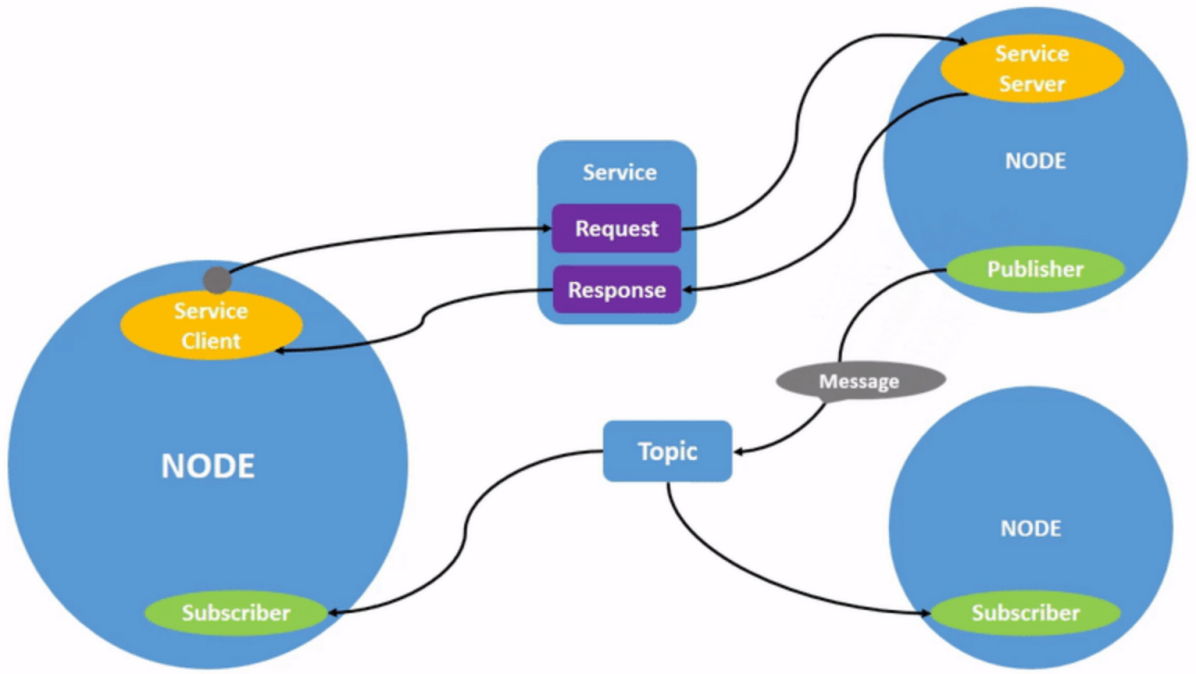
\includegraphics[width=\linewidth]{figs/theory/ros2_node2_01.png} 
        \subcaption{Publish message} \label{fig:ros2_node2:Publisher} 
    \end{subfigure} 
    \vspace{0.5cm}
    \begin{subfigure}[t]{0.9\textwidth} 
        \centering 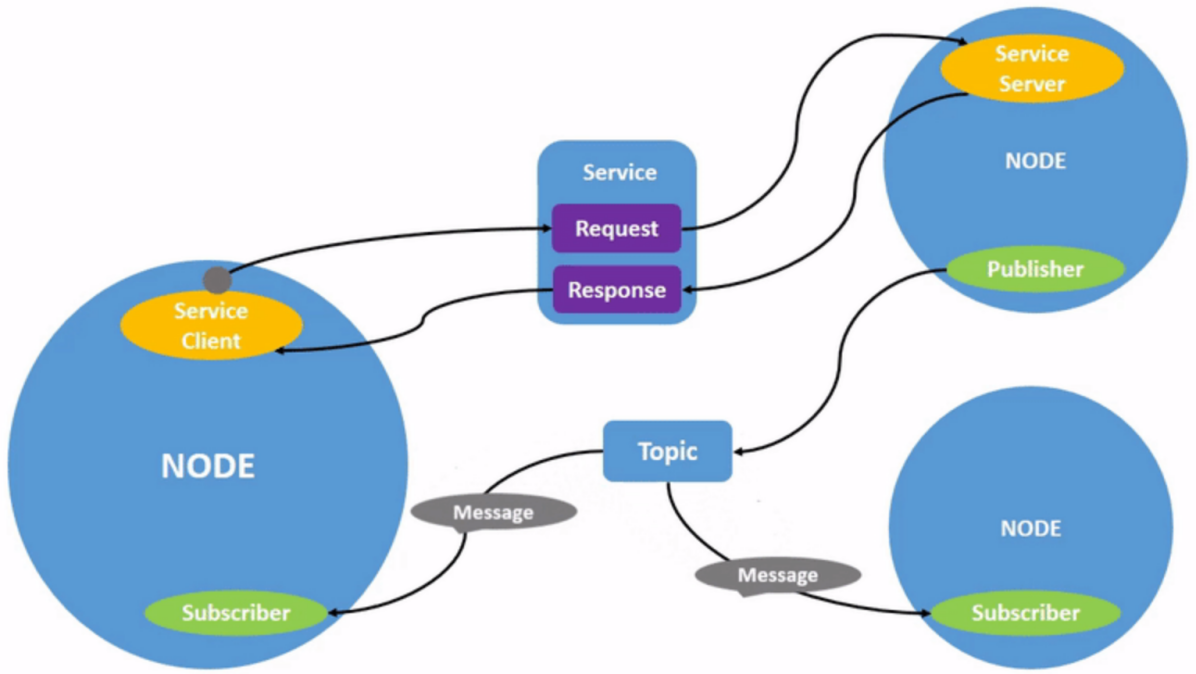
\includegraphics[width=\linewidth]{figs/theory/ros2_node2_02.png} 
        \subcaption{Subscribe messages} \label{fig:ros2_node2:Subscribers} 
    \end{subfigure} 
    \caption{ROS2 Nodes (Publisher) \& (Subscribers)} 
    \label{fig:ros2_nodes} 
\end{figure}

A full robotic system is comprised of many nodes working in concert. In ROS 2, a single executable (C++ program, Python program, etc.) can contain one or more nodes. A node is a fundamental ROS 2 element that serves a single, modular purpose in a robotics system.

\subsection{Topic}
\label{sec:ros2_topic}
ROS 2 breaks complex systems down into many modular nodes. Topics are a vital element of the ROS graph that act as a bus for nodes to exchange messages. As shown in Figure~\ref{fig:ros2_topics}, nodes can publish messages to a topic, and other nodes can subscribe to that topic to receive those messages. This allows for a flexible and decoupled communication mechanism between nodes. A node may publish data to any number of topics and simultaneously have subscriptions to any number of topics.
Topics are one of the main ways in which data is moved between nodes and therefore between different parts of the system.

\begin{figure}[htbp] 
    \centering 
    \begin{subfigure}[t]{0.9\textwidth} 
        \centering 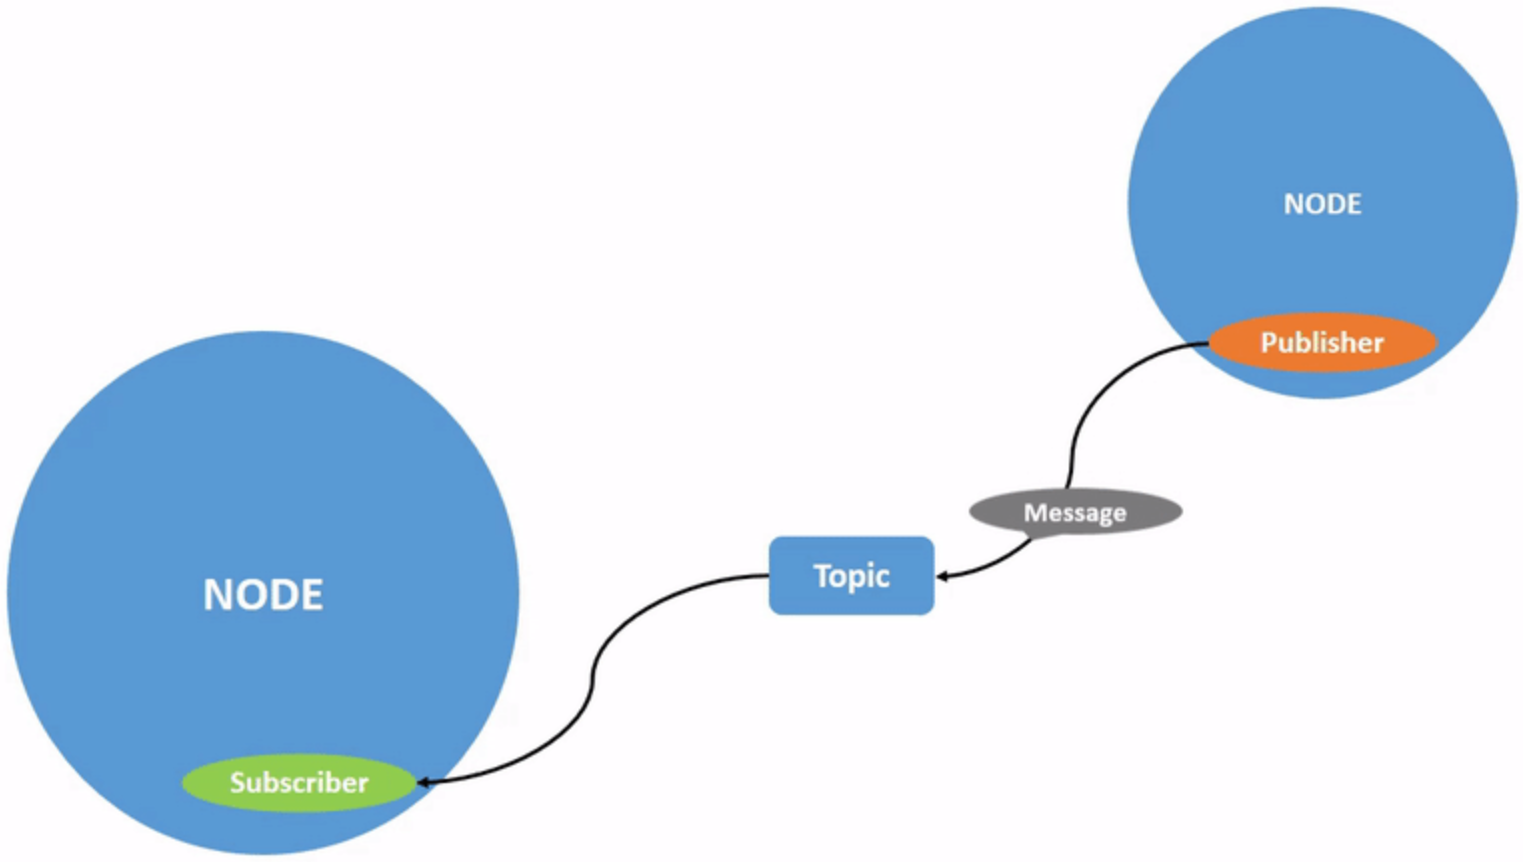
\includegraphics[width=\linewidth]{figs/theory/ros2_topic_01.png} 
        \subcaption{one-to-one} \label{fig:ros2_node2_one2one} 
    \end{subfigure} 
    \vspace{0.5cm}
    \begin{subfigure}[t]{0.9\textwidth} 
        \centering 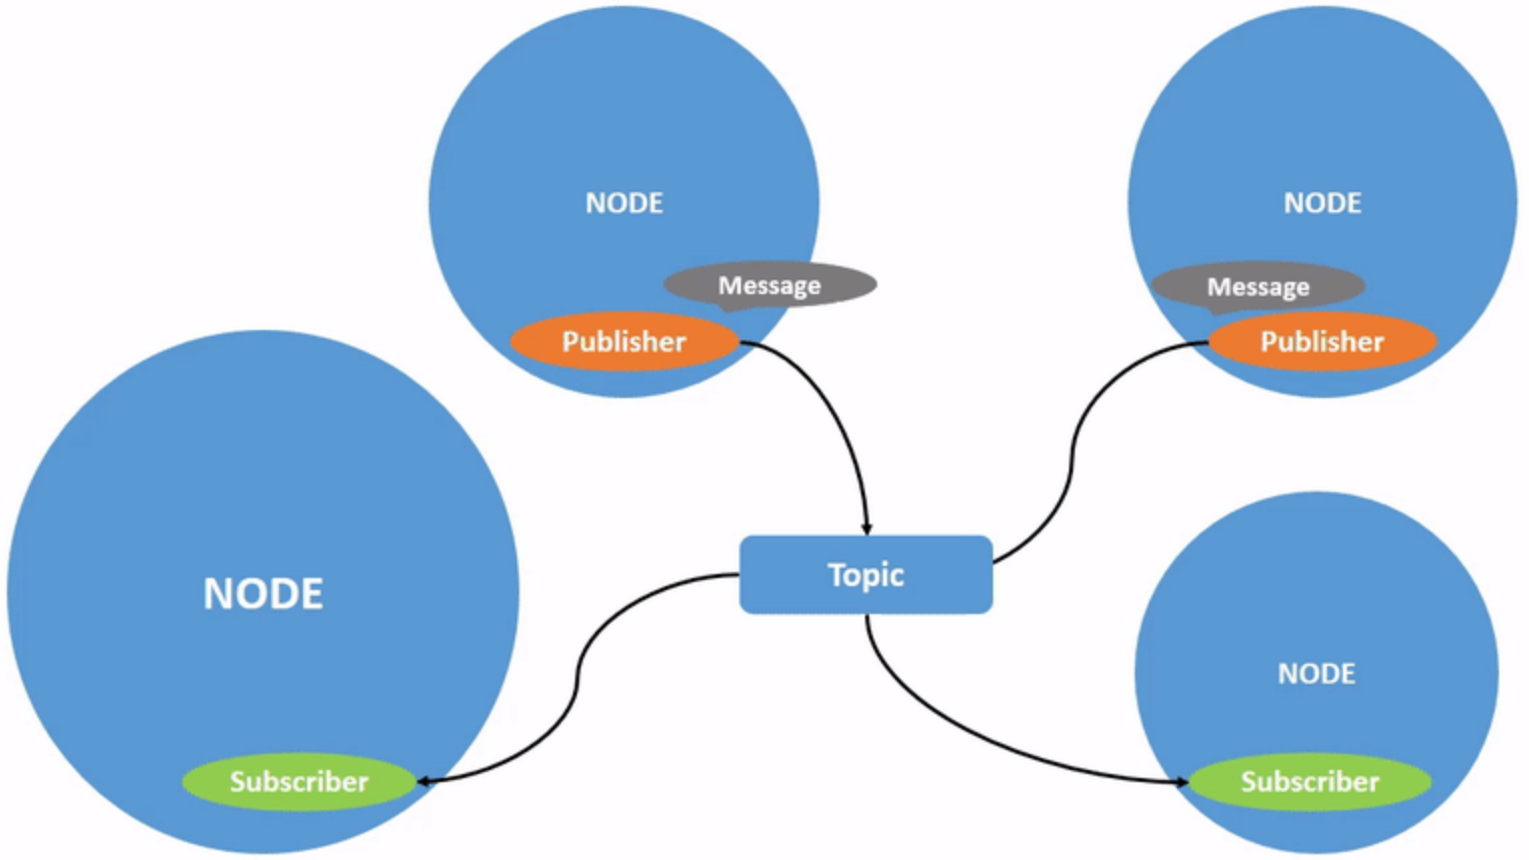
\includegraphics[width=\linewidth]{figs/theory/ros2_topic_02.png} 
        \subcaption{many to many} \label{fig:ros2_node2_many2many} 
    \end{subfigure} 
    \caption{ROS2 Topics (one-to-one) \& (many to many)} 
    \label{fig:ros2_topics} 
\end{figure}

\subsection{Service}
\label{sec:ros2_service}
Services are another method of communication for nodes in the ROS graph. Services are based on a call-and-response model versus the publisher-subscriber model of topics. While topics allow nodes to subscribe to data streams and get continual updates, services only provide data when they are specifically called by a client.
\begin{figure}[htbp] 
    \centering 
    \begin{subfigure}[t]{0.9\textwidth} 
        \centering 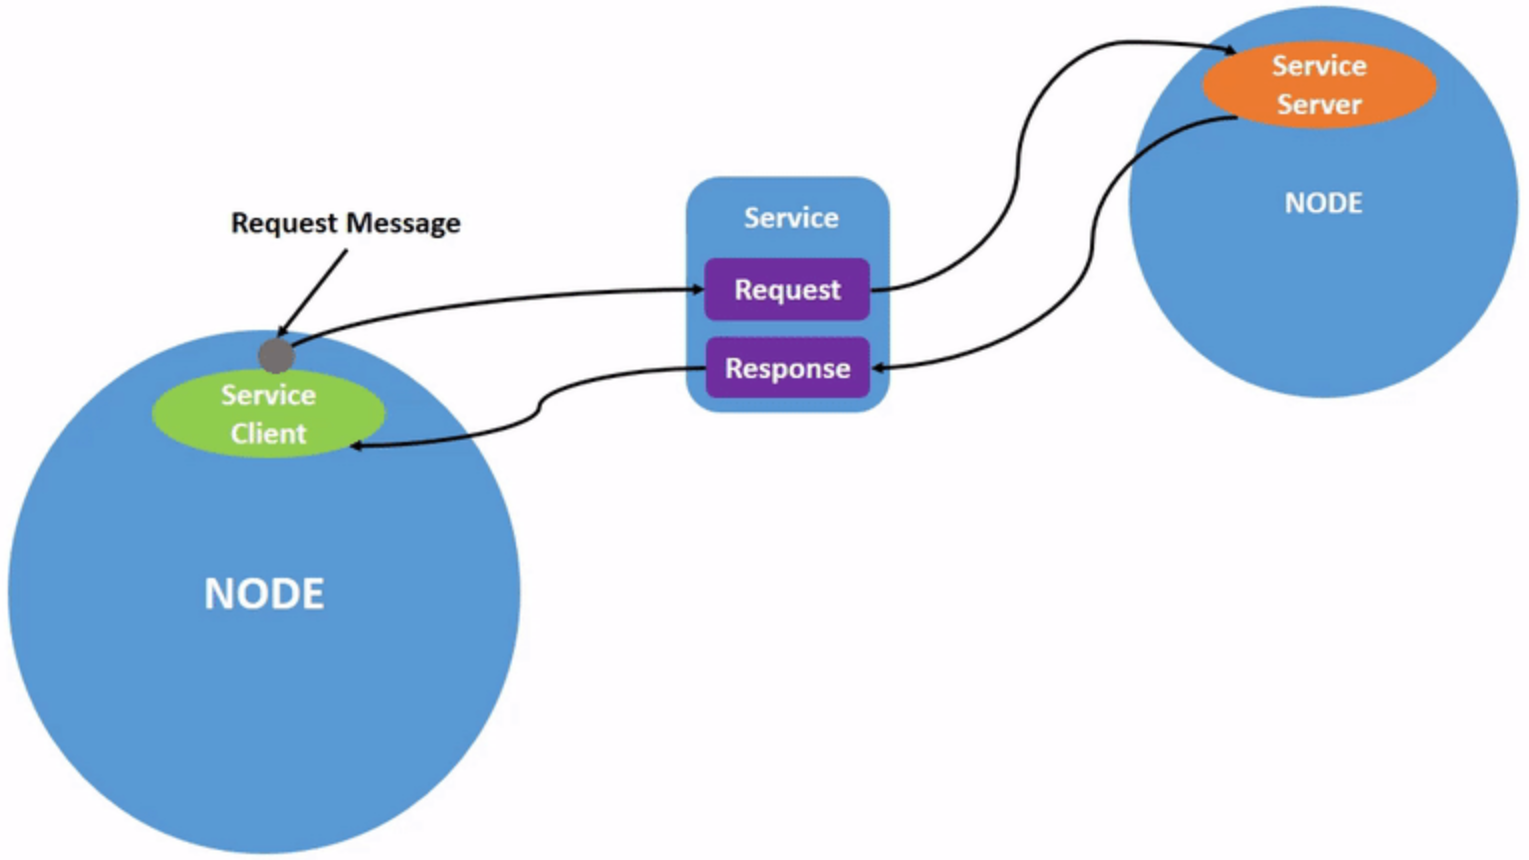
\includegraphics[width=\linewidth]{figs/theory/ros2_service_01.png} 
        \subcaption{one-to-one} \label{fig:ros2_service_one2one} 
    \end{subfigure} 
    \vspace{0.5cm}
    \begin{subfigure}[t]{0.9\textwidth} 
        \centering 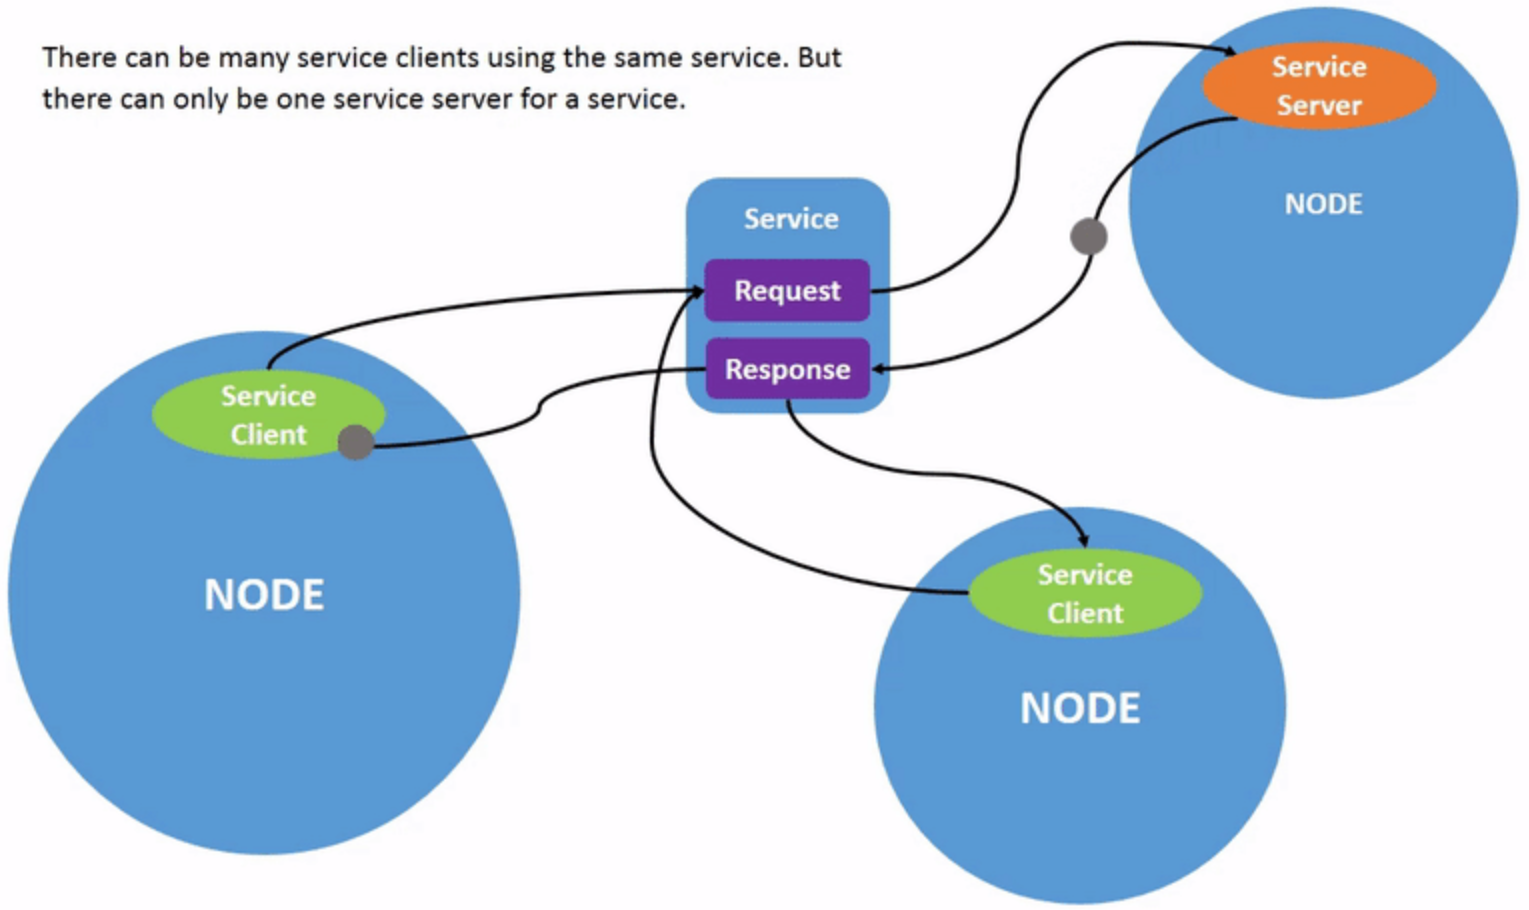
\includegraphics[width=\linewidth]{figs/theory/ros2_service_02.png} 
        \subcaption{many to one} \label{fig:ros2_node2_many2one} 
    \end{subfigure} 
    \caption{ROS2 Services (one-to-one) \& (many to one)} 
    \label{fig:ros2_services} 
\end{figure}
Nodes can communicate using services in ROS 2. Unlike a topic - a one way communication pattern where a node publishes information that can be consumed by one or more subscribers - a service is a request/response pattern where a client makes a request to a node providing the service and the service processes the request and generates a response.

\subsection{Action}
Actions are one of the communication types in ROS 2 and are intended for long running tasks. They consist of three parts: a goal, feedback, and a result.

As shown in Figure~\ref{fig:ros2_action}, actions are built on topics and services. Their functionality is similar to services, except actions can be canceled. They also provide steady feedback, as opposed to services which return a single response. 

Actions use a client-server model, similar to the publisher-subscriber model (described in the section~\ref{sec:ros2_topic}). An “action client” node sends a goal to an “action server” node that acknowledges the goal and returns a stream of feedback and a result.

\begin{figure}[htbp]
    \centering
    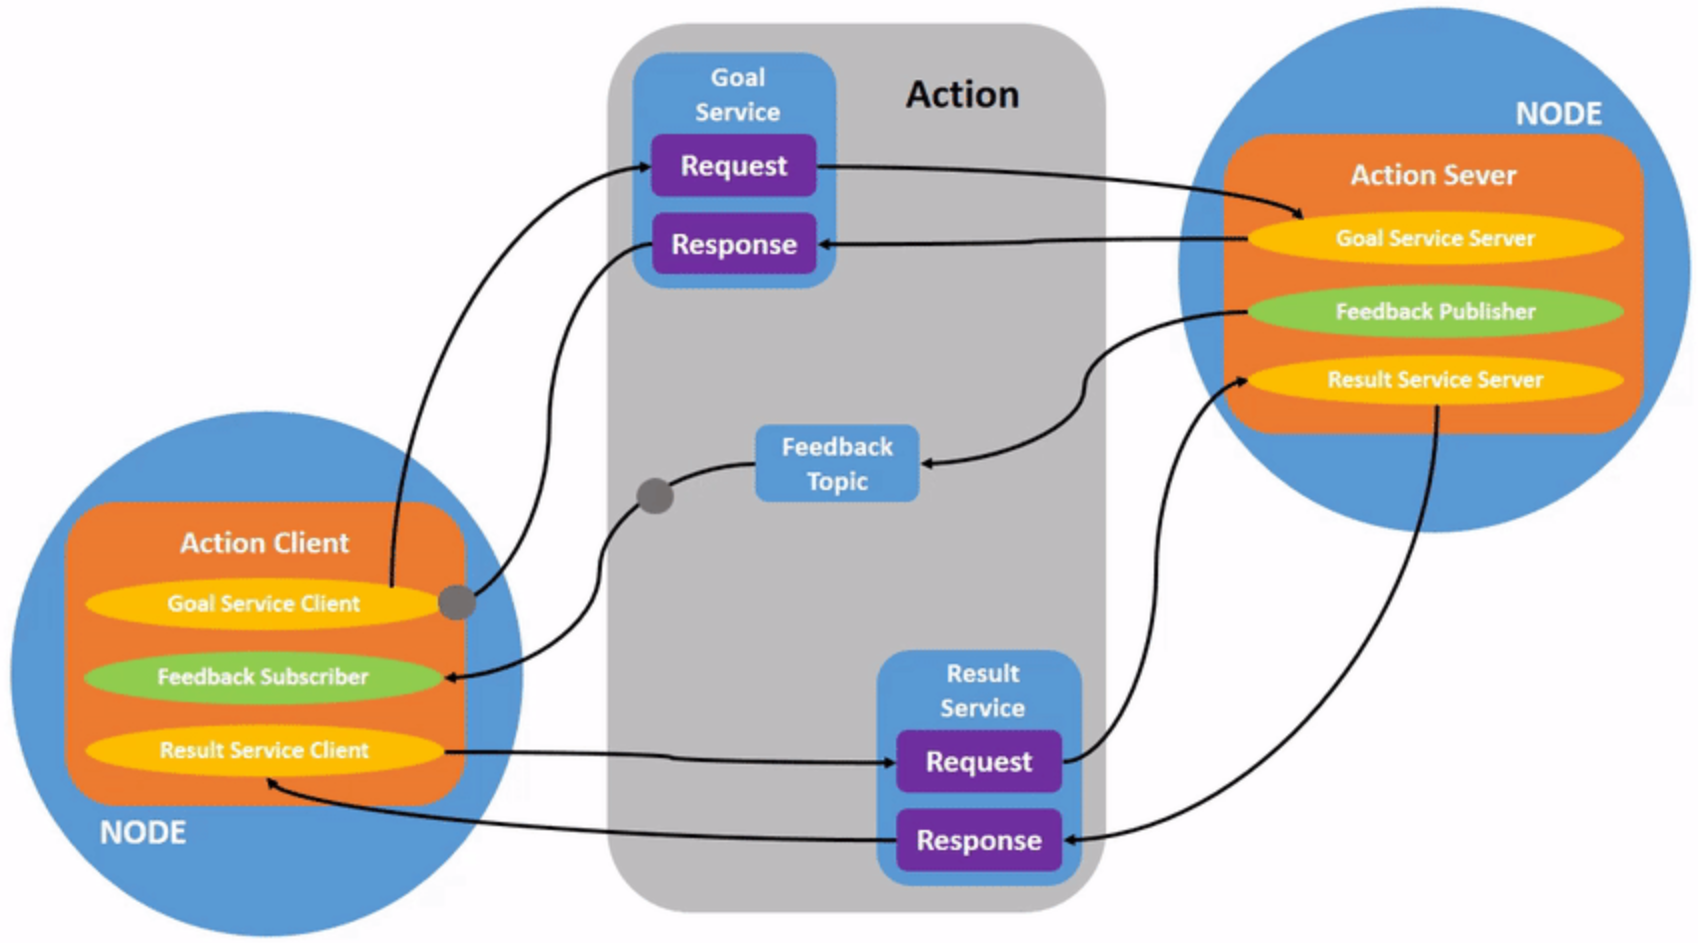
\includegraphics[width=0.9\textwidth]{figs/theory/ros2_action.png}
    \caption{ROS2 Action}
    \label{fig:ros2_action}
\end{figure}

A robot system would likely use actions for navigation. An action goal could tell a robot to travel to a position. While the robot navigates to the position, it can send updates along the way (i.e. feedback), and then a final result message once it’s reached its destination.

\subsection{Parameter}
\label{sec:ros2_parameter}
A parameter is a configuration value of a node. You can think of parameters as node settings. A node can store parameters as integers, floats, booleans, strings, and lists. In ROS 2, each node maintains its own parameters.

Nodes have parameters to define their default configuration values. You can get and set parameter values from the command line. You can also save the parameter settings to a file to reload them in a future session.

\subsection{TF2}
\label{sec:ros2_transform}
tf2 is the second generation of the transform library, which lets the user keep track of multiple coordinate frames over time. tf2 maintains the relationship between coordinate frames in a tree structure buffered in time, and lets the user transform points, vectors, etc between any two coordinate frames at any desired point in time.

Figure~\ref{fig:tf2_vslam_tree} shows the tf2 tree structure used in this engineering project. The root frame is the \texttt{map} frame, which is the global coordinate frame of the environment. The \texttt{odom} frame is the odometry frame, which is used to track the robot's position and orientation over time. The \texttt{zed\_camera\_link} frame is the robot's base frame, which is used to represent the robot's position and orientation in the environment. The \texttt{zed\_left\_camera\_frame} and \texttt{zed\_right\_camera\_frame} frames are the left and right camera frames, respectively, which are used to represent the stereo camera's position and orientation.

\begin{figure}[htbp]
    \centering
    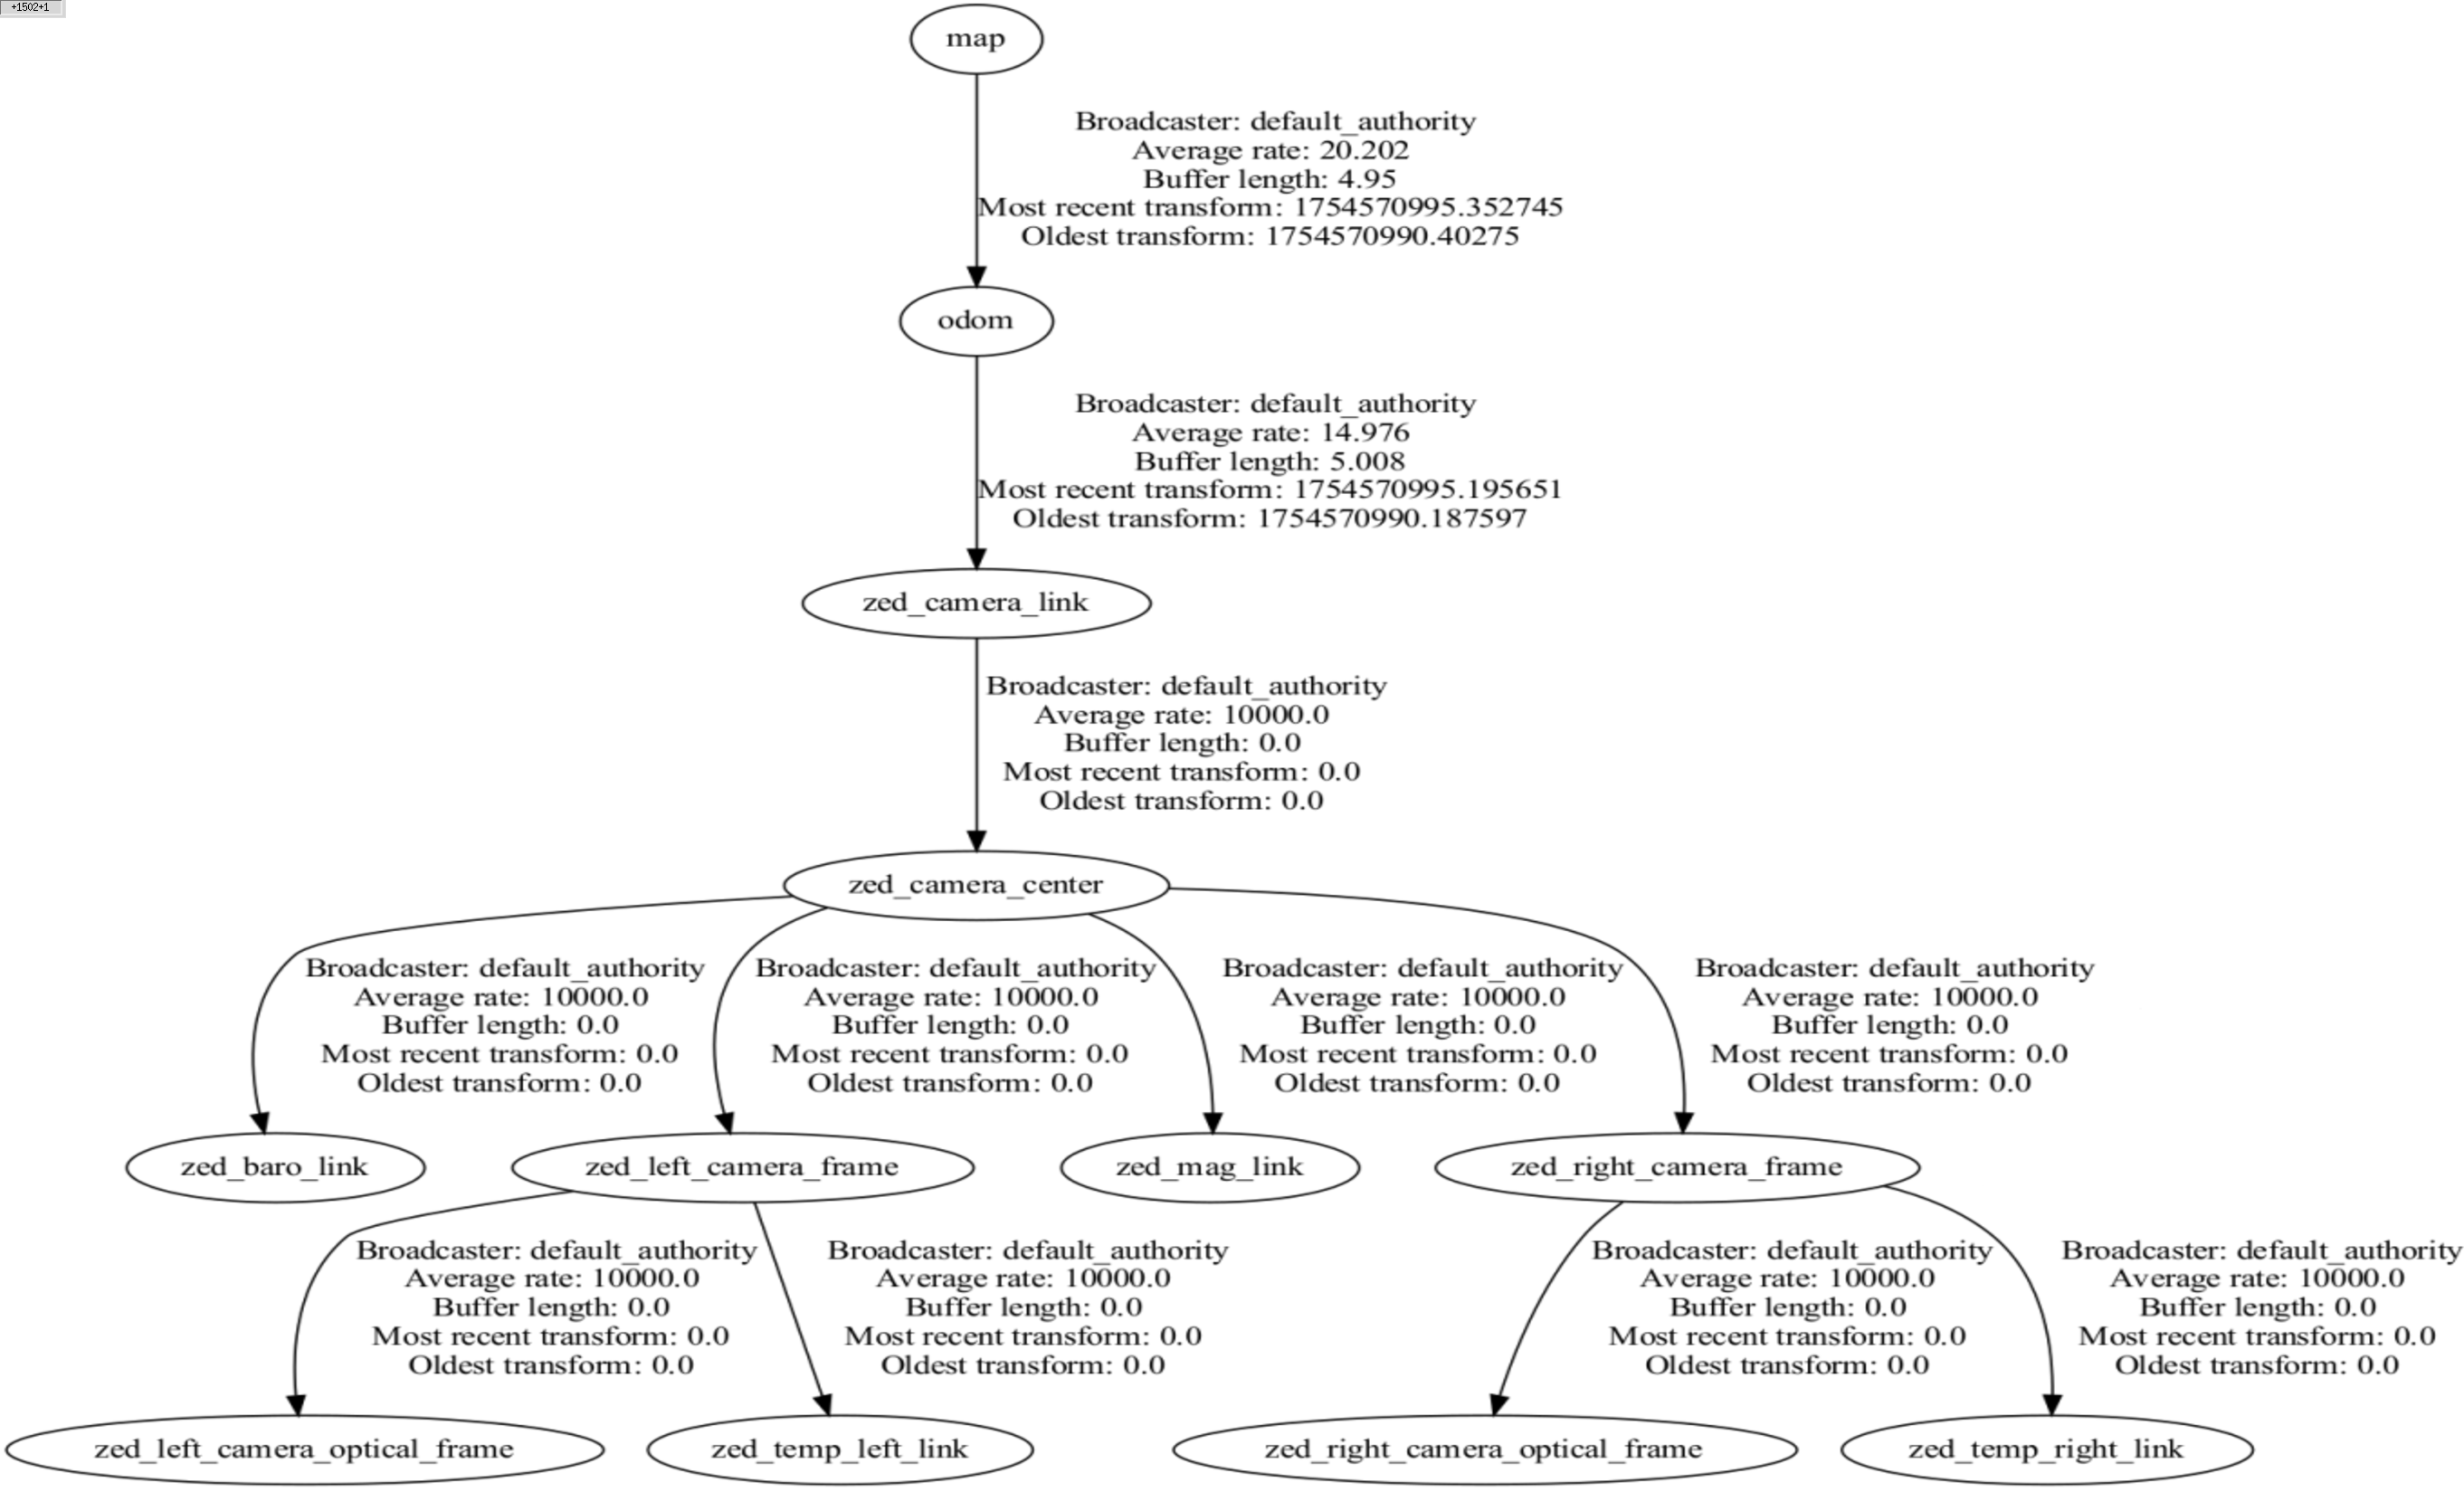
\includegraphics[width=0.9\textwidth]{figs/theory/tf2_vslam_tree.png}
    \caption{TF2 tree structure used in this engineering project.}
    \label{fig:tf2_vslam_tree}
\end{figure}

